\documentclass[11pt,twocolumn]{witseiepaper}
\RequirePackage{ifpdf}
\usepackage{amsmath}
\usepackage{amssymb}
\usepackage{KJN}
\usepackage{pdfpages}
\renewcommand*{\bibfont}{\small}

\ifpdf
\pdfinfo{
	/Title (Research Proposal)
	/Author (Alice Yang (597609))
}
\fi

\begin{document}
	\title{Masters Research Proposal - What are the effects of implementing a two-step system that includes a dimensionality reduction process for the detection of bone fractures }
	
	\author{Alice Yang (597609) \thanks{School of Electrical and Information Engineering, University of the Witwatersrand, Private Bag 3, 2050, Johannesburg, South Africa} }
	
	\abstract{The objective of this paper is to propose a two-step system for the detection of bone fractures in order to investigate the performance of the system compared to a single step system. The performance are defined by the speed of its execution, classification accuracy and error rate. The two-step system consists of a dimensionality reduction and a automated decision making process. The objective of the introduction of the dimensionality reduction process is to improve the performance of the automated decision making process during the training and decision making sessions. }
	
	\keywords{Dimensionality Reduction, Neural Networks, Supervised Learning,  Unsupervied Learning, Bone Fractures, Medical Images}
	\maketitle
	\thispagestyle{empty}\pagestyle{empty}
	
	\section{Introduction}
	In medical the field there is an emphasis on the importance of medical diagnosis. In critical cases, an inaccurate diagnosis of a symptom can cost a patient's life. Many diagnosis are performed by trained medical doctors, however they are prone to making mistakes which can be influenced by external factors, such as fatigue and lack of training in the particular field. Automation of medical diagnosis was introduced in the early 1970s \cite{Ramesh2004}. There are many algorithms available in diagnosing patients. The basic algorithm consists of "if... then..." statements. Although the algorithm is simple, the list of conditions in the medical field are endless and as a result the execution time to diagnosis a patient's symptoms is not realistic. There are many pattern recognition algorithms available which are categorized in two categories, namely, unsupervised and supervised. The reasoning behind making use of artificial intelligence is to reduce costs. In this proposal report, section 2 presents the background in the related topics, section 3 describes the problem, section 4 illustrates the proposal methodology, section 5 shows the time management for the proposed research and section 6 concludes the paper.
	
	\section{Background}
	There are many simple implementations of programs that are proposed to diagnosis common medical conditions. These implementations requires a vast majority of the medical knowledge to express the different descriptions of possible diseases to be stored in the program's database. Although the program is simple to implement, it has no method of measuring the severity of the patient's illness. Another downfall to using a database to diagnosis an illness, is that it can mean that the database can grow exponentially otherwise it would be outdated. 
	
	An alternative approach in medical diagnosis is to focus on one disease to ensure accuracy and quick response. The use of artificial intelligences can be focussed in one area. The focus of this paper is to detect bone fractures from X-Ray images. There are a selection of tools that can be applied in order to achieve the desired outcome for this investigation. These tools can be in the form of supervised learning, reinforcement, unsupervised learning or a combination of the two. Support Vector Machine and Neural Networks are common tools used in artificial intelligence (AI).
	
	\section{Literature Review}
	The review done by \cite{Mahendran2011} for the automation of bone fracture detection indicated that there are various techniques in pattern recognition that comes in the form of unsupervised, reinforcement and supervised. The challenge found in classification are that there is an information overload and size and dimension are a concern. The problem with information overload is that it becomes to computationally expensive to find crucial information needed for the classification. The size and dimension of the information is a concern because large sizes of data contributes to the number of dimensionality, with high number of dimensions it presents a challenge in the classification process and in turn may require more computational resources.
	
	\subsection{\textbf{Unsupervised Learning}}
	Unsupervised learning is defined by the not needing to train the algorithm in order for it to classify data into different categories. This process allows the algorithm to learn more about the given data. There are two categories in unsupervised learning which are clustering and association. Popular unsupervised algorithms are k-means and Apriori algorithm. The clustering technique is an example of un-supervised learning, since the technique analyses a given set of data and groups the data that have similar characteristics together. One of the main advantages of clustering is that it is adaptable when given new data sets compared to classification. It is also useful for singling out useful features. There are various types of clustering methods, namely, partitioning, hierarchical, density-based, grid-based, model-based and constraint-based. Other unsupervised learning techniques includes Principal Component Analysis, Independent Component Analysis, Non-Negative Matrix Factorization and Singular Value Decomposition. 
	
	\subsection{\textbf{Dimensionality Reduction}}
	The collection of digital data has increased drastically over the past decade, which led to datasets having high dimensionality. The high dimensionality found in datasets affected the performance of data processing algorithms. This is known as the curse of dimensionality \cite{Center2002}. Dimensionality reduction is a process targeted at reducing the dimensionality of the considered dataset by reducing the number of random variables. This process can be divided into two stages, namely Feature Selection and Feature Extraction. Both these stages are crucial for automating bone fracture detection. There are two types of dimensionality techniques, convex and concave techniques. This section focuses on convex techniques. Convex techniques optimizes objective functions that do not contain any local optima, which means that the solution space is convex \cite{Boyd2010}. The objective function is usually in a generalized Rayleigh quotient, which can be expressed in the following form: 
	\begin{equation}
	\phi(\textbf{Y}) = \frac{\textbf{Y}^{T}\textbf{AY}}{\textbf{Y}^{T}\textbf{BY}}
	\label{eq: general objective function}
	\end{equation}
	The function expressed in the form of Equation \ref{eq: general objective function} can be easily optimized by solving a generalized eigenproblem. Convex dimensionality reduction techniques can be subdivided into techniques that perform eigendecomposition on full matrix and sparse matrix. The following section focuses on the eigendecomposition of full matrix. 
	
	\subsubsection{PCA/Classical Scaling}
	Principal Component Analysis (PCA) is a linear technique that performs dimensionality reduction through the process of embedding the data into a linear subspace of low-dimensionality. The low-dimensional representation of the data describes the variance of the data \cite{Jolliffe2016}. During the construction of the low-dimensional representation, PCA does not discard information, instead it creates new characteristics to represent the original characteristics. This is done by searching for characteristics that show as much variation as possible. Additionally, PCA searches for characteristics that allows for the reconstruction of the original characteristics from the new characteristics. According to \cite{van2009dimensionality}, maximizing the variance will result to minimizing the error. Hence, the construction of the low-dimensional representation is obtained by determining mapping  \textbf{M} which maximizes the cost function. The cost function is expressed in Equation \ref{eq: scaling cost function}.
	\begin{equation}
	\phi(\textbf{Y}) = \sum_{ij}(d_{ij}^{2} - ||\textbf{y}_i - \textbf{y}_j||^2)
	\label{eq: scaling cost function}
	\end{equation}
	where 
	
	$||\textbf{y}_i - \textbf{y}_j ||^{2}$ = squared Euclidean distance between low-dimensional datapoints $\textbf{y}_i$ and $\textbf{y}_j$
	
	Eigenvectors and eigenvalues are solved using the eigenproblem expressed in Equation \ref{eq: eigenproblem}. Eigenvectors and eigenvalues are crucial in PCA since eigenvectors assist with determining the correlation between the data points whilst eigenvalues, $\lambda$ dictates the weighted average of the variance for any projection.
	\begin{equation}
	cov(\textbf{X})\textbf{M} = \lambda\textbf{M}
	\label{eq: eigenproblem}
	\end{equation}
	The disadvantage with PCA is that the size of the covariance matrix is dependent on the dimensionality of the original dataset. This means that the size of the covariance matrix is proportional to the number of dimensionalities presented by the dataset, which can result in the inability to compute eigenvectors for very high-dimensional datasets \cite{van2009dimensionality}.
	
	Classical Scaling is an identical technique to PCA, however Classical Scaling searches for the linear mapping \textbf{M} that minimizes the cost function that is expressed in Equation \ref{eq: scaling cost function}. Furthermore, the low-dimensional representation is of the Gram Matrix in which the double-centering pairwise squared Euclidean distance matrix entries are obtained using Equation \ref{gram_enteries}.
	\begin{equation}
	k_{ij} = -\frac{1}{2}(d_{ij}^{2}-\frac{1}{n}\sum_{l}d_{il}^{2} - \frac{1}{n}\sum_{l}d_{jl}^{2} + \frac{1}{n^2}\sum_{lm}d_{lm}^{2})
	\label{gram_enteries}
	\end{equation}
	The disadvantage for both PCA and Classical Scaling is the cost function in Equation \ref{eq: scaling cost function} focuses on retaining large pairwise distances $d_{ij}^2$, whereas retaining the small pairwise distance can be important for minimizing error.
	
	\subsubsection{Isomap}
	Unlike PCA and Classical Scaling where the aim of the techniques is to retain the pairwise Euclidean distances, the Isomap technique attempts to preserves the pairwise
	geodesic distances between datapoints \cite{Zhang2012}. This means that the geodesic distance between $x_i$ and $x_j$ imitates as much of the Euclidean between the low-dimensional representation yi and yj as possible. The low-dimensional representation $y_i$ and $y_j$ are computed using the classical scaling technique, which results in a pairwise geodesic distance matrix. The drawback of the Isomap technique is that it constructs erroneous connections in the neighbourhood graph, G which can affect the performance of the Isomap.
	
	\subsubsection{Kernel PCA}
	Kernel Principal Component Analysis (KPCA) is a technique that makes use kernel functions to map data into high dimensional space, by which the space is manipulated using linear PCA \cite{Cui2012}. KPCA makes use of a mapping function by which it computes the kernel matrix $K$ of datapoints $x_i$ and $x_j$. The enteries for the kernel matrix is defined by Equation \ref{eq: kernel matrix enteries}.
	\begin{equation}
		k_{ij} = K(x_i, x_j)
		\label{eq: kernel matrix enteries}
	\end{equation}
	where
	\begin{align*}
		K &= \text{kernel function}\\
		x_i \text{ and } x_j &= \text{input datapoints}
	\end{align*}
	The features defined by the kernel function have a zero-mean. Additionally, the eigenvectors of the covariance matrix $\textbf{a}_i$ which is expressed in Equation \ref{eq: kernel covariance matrix} can be computed, since the eigenvectors of the kernel matrix are related.
	\begin{equation}
		\textbf{a}_i = \frac{1}{\sqrt{\lambda_i}} \textbf{v}_i
		\label{eq: kernel covariance matrix}
	\end{equation}
	The low-dimensional representation is obtained by the projection given by Equation \ref{eq: kernel low-dimensional}.
	\begin{equation}
		\textbf{y}_i = \left\{ \sum_{j = 1}^{n}a_1^{(1)}K(\textbf{X}_j, \textbf{X}_i), ... , \sum_{j = 1}^{n}a_d^{(j)}K(\textbf{X}_j, \textbf{X}_i) \right\}
		\label{eq: kernel low-dimensional}
	\end{equation}
	where
	\begin{align*}
		a_1^{(j)} &= \text{jth value in vector }\textbf{a}_1\\
		K &= \text{kernel function}
	\end{align*}
	A disadvantage with KPCA is that the size of the kernel matrix is proportional square number of instances in the dataset. However despite the obvious disadvantages, KPCA is applied to facial recognition, speech recognition and novelty detection \cite{van2009dimensionality}.
	
	\subsubsection{MVU}
	Maximum Variance Unfolding (MVU) is a technique that aims to preserve as much of the distances and angles between nearby points by studying the kernel matrix. As result it forms a neighbourhood graph, $G$ \cite{Jiang2011}. A quadratic equation is formulated for the "unfolding" transformation. The "unfolding" transformation is where MVU maximizes the sum of the squared Euclidean distances between all the datapoints whilst preserving the distances within neighbouring points. This can be described in Equation \ref{eq: optimization problem}.
	\begin{equation}
		\text{Maximize } \sum_{ij}||\textbf{y}_i - \textbf{y}_j||^{2}
		\label{eq: optimization problem}
	\end{equation}
	\begin{align*}
		\text{Subject to:}
		\begin{cases}
			(1)||\textbf{y}_i - \textbf{y}_j||^{2} = ||\textbf{x}_i - \textbf{x}_j||^{2} , \eta_{ij} = 1 \\
			(2)\sum_{i}\textbf{y}_i = 0
		\end{cases}
	\end{align*}
	MVU reformulates the optimization as semidefinite programming (SDP) over matrix $\textbf{K}$ by defining the inner product of $\textbf{K}_{ij} = \textbf{y}_i \cdot \textbf{y}_j$. Thus the SDP can be written as follows: 
	\newline
	Maximize trace(\textbf{K}) subjected to:
	\begin{equation}
		\begin{cases}
			(1) \textbf{K} \geq 0 \\
			(2) \sum_{ij} \textbf{K}_{ij} = 0 \\
			(3) \textbf{K}_{ii} - 2\textbf{K}_{ij} + \textbf{K}_{jj} = ||\textbf{x}_i - \textbf{x}_j||^{2}, \eta_{ij} = 1
		\end{cases}
	\end{equation} 
	From the first condition $\textbf{K} \geq 0$, it indicates that matrix $\textbf{K}$ is required to be positive semi-definite, since SDP is convex.
	
	Similar to PCA, Independent Component Analysis (ICA) is a technique which analyses data of multidimensional high order. It identifies the independent implicit information in order to remove redundant as well as extract independent information \cite{7852869}. 
	
	Kernel Principal Component Analysis (KPCA) is again similar to the regular PCA, however the difference lies in its application in which KPCA is applied in a none-linear manner. As a result, it creates a none-linear mapping scheme to maximize the variance within the considered data \cite{KPCA_2016}.
	
	Graph-Based Kernel Principal Component Analysis are techniques that are prominent none-linear techniques that makes use of a cost function to construct a low-dimensional representation of the considered data. Such techniques includes Locally Linear Embedding (LLE), Hessian LLE, Laplacian Eigenmaps and Local Tangent Space Alignment (LTSA). 
	
	Linear Discriminant Analysis (LDA)  is a method that finds linear combinations of features that can be characterized two or more classes. It is commonly used in statistics, pattern recognition and machine learning \cite{LDA_2016}.
	
	General Discriminant Analysis (GDA) is similar to LDA in terms of its objectives, in which it is to find crucial features in the considered data such that it lowers the dimensionality of the data. GDA operates with non-linear discriminants by which it makes use of a kernel function. Its underlying theory is similar to that of support vector machine (SVM).
	
	\subsubsection{\textbf{Supervised Learning}}
	The goal of supervised learning to to create a mapping function, such that when given new input data a prediction of the output data can be made. The mapping function is generated by with given data sets that consists of inputs with its corresponding outputs. Linear regression, random forest and SVM are popular supervised algorithms.
	Support Vector Machine (SVM) is a classifier mainly used for complex classification purposes. In order to separate new data into specified categories, SVM is trained with given labelled data making it supervised learning \cite{Rebentrost2014}. An implementation of SVM classifiers is done in \cite{saha_classifying_2016} where the it is used to classify X-Ray images of the body into five categories, namely, head-neck, body, upper-limb and true-negative. Spatial Pyramid Histogram are used to decipher the medical images which is then used to train the Chi-Kernel based SVM. In general, SVM is used for binary classification \cite{Rebentrost2014}.
	
	Neural Networks in another common tool selection for AI, whereby it consists of three distinguished layers, the input, hidden and output layer. A general neural network consists of one or two hidden layers. The network is trained before use, which deems it as supervised classification or predictions. In \cite{jyothi_congenital_2016}, the technique implemented is back-propagation neural network (BPNN). The network is trained using a Supervised Delta Learning Rule. The result from the developed technique is a binary outcome in which it indicates whether the subject is normal or abnormal.
	
	Studies of improving the common tools in AI have been done by combining the tools. There are two types of combinations, hybrid and non-hybrid multiple classifiers. Hybrid multiple classifiers combines different types of AI algorithms, whereas non-hybrid multiple classifiers only consists of one base algorithm and is replicated multiple times. A hybrid multiple classifier is done by \cite{multiple_classification}, in which the algorithms used are K-Nearest Neighbour, Back Propagation Neural Network (BPNN) and SVM. According to the authors, the each of the AI tools is trained with a different set of data. The decision is based on a voting scheme that is called fusion selection. However, the paper presented in \cite{multiple_classification} performs binary results. In other words, it indicates whether a fracture is present or absent. 
	
	Another AI algorithm to be considered for medical diagnosis is deep learning. According to the author in \cite{LeCun2015}, deep learning has the ability to combat complex problems whereas SVM would not be able to, since SVM works better with small data sets that have few outliers. However, the downfall of deep learning is its learning process, in which it can become tedious and computational demanding. Thus for small data sets, it is more plausible to use an off-shelf classifier such as SVM. 
	
	\subsubsection{\textbf{Curse of Dimensionality}}
	The main problematic factor affecting the performance in classification is the curse of dimensionality. The curse of dimensionality is a problem due to the sparsity of high dimensional spaces, in which an absurd amount of training data is needed in order to get low variance  estimators \cite{intrator_feature_1992}.
	
	Feature extraction with supervised learning algorithms may seem most desired compared to unsupervised learning algorithms, since supervised learning algorithms have more information about the problem and features. However, unsupervised methods do not suffer the curse of dimensionality as supervised learning does since it makes use of local measures to optimally estimate a single dimensional projection function \cite{intrator_feature_1992}.
	
	\subsubsection{\textbf{Combination Techniques}}
	There have been studies done which combine the algorithms of supervised and unsupervised. The authors of \cite{neagoe_new_2014} proposed a method which combines both supervised and unsupervised algorithms, name.
	
	The authors of \cite{kottaimalai_eeg_2013} designed a system in which it comprises of Principal Component Analysis(PCA) and Neural Network for the classification of EEG Signals. PCA is a form of unsupervised learning whilst neural network is supervised learning and requires training. The authors compared the correctness of the classification using Neural Network to using Principal Component Analysis with Neural Network. The final outcome from the experimentation is that the correctness of the classification of the Principal Component Analysis with Neural Network is better than Neural Network alone. 
	
	\section{Problem Analysis}
	The modern world has presented the technology to predict human speech as well as digitally categorizing handwritten numbers. However, this technology has not been fully utilized in the medical field. There are many debates surrounding the topic of whether machines are better than doctors. In many cases, the argument for doctors states that those who develop AI do not understand the complexity of medicine and those arguing for the machines say that not many understand how AI operates. However, at the end of the day there are still sick patients waiting to be treated with the right medication or medical care. In order to determine the type of medical care the patient needs a diagnosis must be performed. According to \cite{meyer_physicians_2013}, where studies have been done around the United States, it was reported that doctors correctly diagnosed 55.3\% for easier cases and 5.8\% for more difficult cases. However, this is only one article and more investigation is needed to confirm these numbers. Even so, these numbers still indicate that doctors are not perfect and can mis-diagnosis patients. As a result of mis-diagnosis, the patient is subjected to stress or even life threatening situations should the disease be mis-treated. Therefore there is a large emphasis on accuracy and quick detection of diseases.
	
	There are existing pattern recognition techniques available which have the ability to detect the presence of bone fracture. However, there are large amounts of datasets that is passed into the techniques. These datasets create dimensionality, the more datasets there are the higher the number of dimensionality there are. High number of dimensionalities affects the performance of the techniques. This is known as the curse of dimensionality. 
	
	\section{Proposed Methodology}
	The purpose of this research is to develop a system which consists of two steps in order to determine the presence of a fracture with medical x-ray images as the system's input. The first step is a dimensionality reduction process and the second step is the automation of the decision making process. The objective of the dimensionality reduction process is to map the data from a high dimensionality to a low dimensionality without loosing any critical information needed for the decision making process. 
	
	The proposed approach adopted for this research is illustrated in Figure \ref{fig:system overview}. The proposed system consists of an image processing technique, dimensionality reduction and an automated decision making technique. The proposed system mainly focuses on the dimensionality reduction and automated decision making techniques. The objective of the proposed system is to determine the effects of using two steps compared to using one for the detection of bone fracture. The evaluation of the effects of the systems is done by observing the execution speed, classification accuracy and error rate.
	
	\begin{figure}[!h]
		\centering
		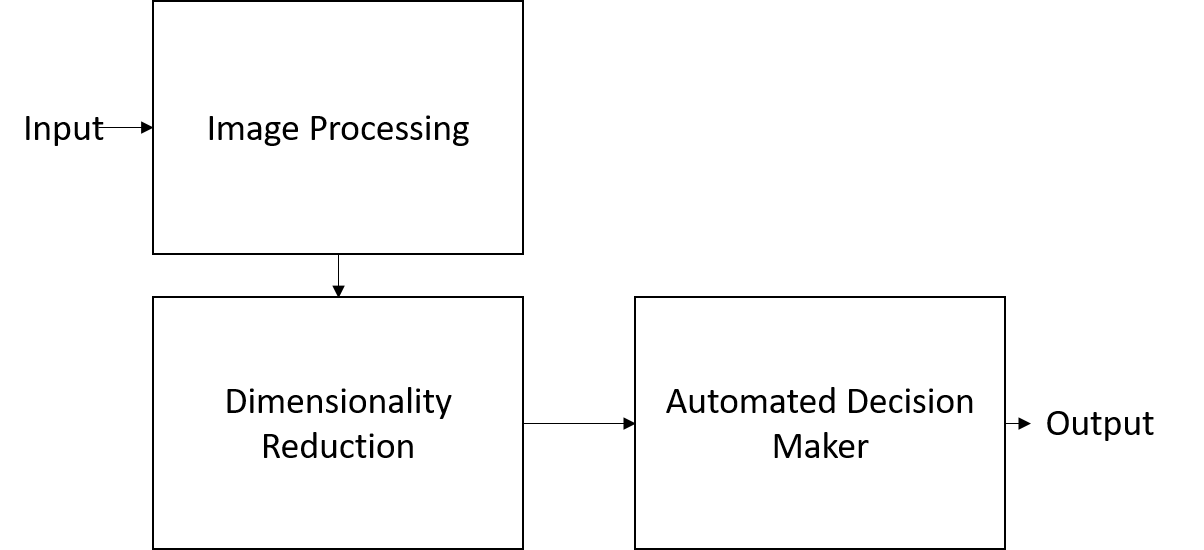
\includegraphics[scale=0.23]{system_overview.png}
		\caption{Block Diagram illustrating an overview of the system }
		\label{fig:system overview}
	\end{figure}
	
	\subsection{Feature Selection}
	Feature selection is performed through the process of image processing, whereby the Canny and Sobel techniques are utilized. The features selected are shown in Table \ref{feature_selection}.
	
	\begin{table}[!h]
		\centering
		\caption{Table showing the selected features and the dimensions of each feature.}
		\label{feature_selection}
		\begin{tabular}{|l|p{2cm}|l|}
			\hline
			Features & No. of Dimension & Description \\
			\hline \hline
			gradient & 2 & hough line value, \\
			& & angle (in degrees)\\
			\hline
			lines    & 4 & $x_{1}$, $y_{1}$ \\
			& & $x_{2}$, $y_{2}$ \\
			\hline
			contours & N  & line values that make \\
			& & up the contour\\
			\hline
		\end{tabular}
	\end{table}
	
	\subsection{Dimensionality Reduction}
	The selected features illustrated in Table \ref{feature_selection} have differing dimensions. The dimensions of the contour feature can vary depending on the type bone presented in the x-ray image. Therefore there is a high dimensionality in the dataset that represents one x-ray image. Although there is enough information from the selected features to represent an x-ray image, there is also redundant information present in the dataset. The automated decision making process has the ability to process the raw data, however in doing so it will hinder its overall performance. The PCA and ICA techniques are under consideration for the dimensionality reduction technique. Therefore it is subjected to change. 
	
	\subsection{Automated Decision Making Techniques}
	The automation of bone fracture detection can be done by utilizing a neural network technique. The implementation of the neural network technique consists of two stages. The first stage is the training of the technique and the second is the classification of the bone fracture. The neural network technique has the ability to process the raw data from the selected features, however since the raw data has high dimensionality it has the potential to hinder the performance of both stages in the neural network technique. This will be observed during execution. The neural network technique in consideration is Back Propagation Neural Network, however this choice of technique is subjected to change.
	
	\section{Time Management}
	Table \ref{time_management} presents the time management for the proposed research presented. 
	\begin{table}[!h]
		\centering
		\caption{Table showing the time management of the implementation of a bone fracture detection two step system.}
		\label{time_management}
		\begin{tabular}{|l|p{5cm}|}
			\hline
			Date & Task \\
			\hline \hline
			1 March & 1st Draft Hand-In \\
			\hline
			2 March & Investigate best suited dimensionality reduction technique for selected features \\
			\hline
			8 March & Present 1st iteration of source code for the two step system \\
			\hline
			15 March & Present 2nd iteration with automated decision making process implemented \\
			\hline
			22 March & Submit Proposal \\
			\hline
		\end{tabular}
	\end{table}
	
	\section{Conclusion}
	To conclude, the system proposed for the detection of bone fracture consists of two steps. The first step is dimensionality reduction and the second step is the automation of decision making. The objective of implementing a dimensionality reduction process is to improve the performance of the automated bone fracture detection. The performance is measured by speed, classification accuracy and error rate. 
	
	\newpage
	\bibliographystyle{witseie}
	\bibliography{standard}
	
\end{document}